% Figure~\ref{fig:Schematic_representation_artificial_neuron}
% (Section 2: "GUM Analytical Law of Propagation of Uncertainty for Deep
% Neural Networks").
%
% Replaces the borrowed image NN_neuron_with_bias.png. Notation as in
% Eqs. (Law_of_Propagation_of_Uncertainty_for_NN) and (H_i_definition):
%   x^(i)   output of layer i, x^(0) = x (input), x^(L) = y (output);
%   W_i, b_i  weight matrix and bias vector of layer i, elements W_{i,jk}, b_{i,j};
%   sigma_i   activation function of layer i, applied elementwise;
%   z_i = W_i x^(i-1) + b_i  preactivation;
%   H_i = diag[sigma_i'(z_i)];
%   U_x^(i) = H_i W_i U_x^(i-1) W_i^T H_i^T.
% (a) artificial neuron j of layer i; (b) MLP with the layer-wise
% covariance propagation underneath.
%
% Compiles with plain pdflatex to a tightly-cropped vector PDF.
% Okabe-Ito colours as in the other figures of the paper.
\documentclass{article}
\usepackage{amsmath}
\usepackage{amssymb}
\usepackage{bm}
\usepackage{tikz}
\usetikzlibrary{arrows.meta, positioning, calc, fit, backgrounds}

\definecolor{okBlue}{HTML}{0072B2}
\definecolor{okOrange}{HTML}{D55E00}
\definecolor{okGreen}{HTML}{009E73}

\pagestyle{empty}
\newsavebox{\figbox}
\newlength{\figborder}
\setlength{\figborder}{4pt}

\newcommand{\vx}{\mathbf{x}}
\newcommand{\vb}{\mathbf{b}}
\newcommand{\mW}{\mathbf{W}}
\newcommand{\mH}{\mathbf{H}}
\newcommand{\mU}{\mathbf{U}}

\begin{document}
\begin{lrbox}{\figbox}%
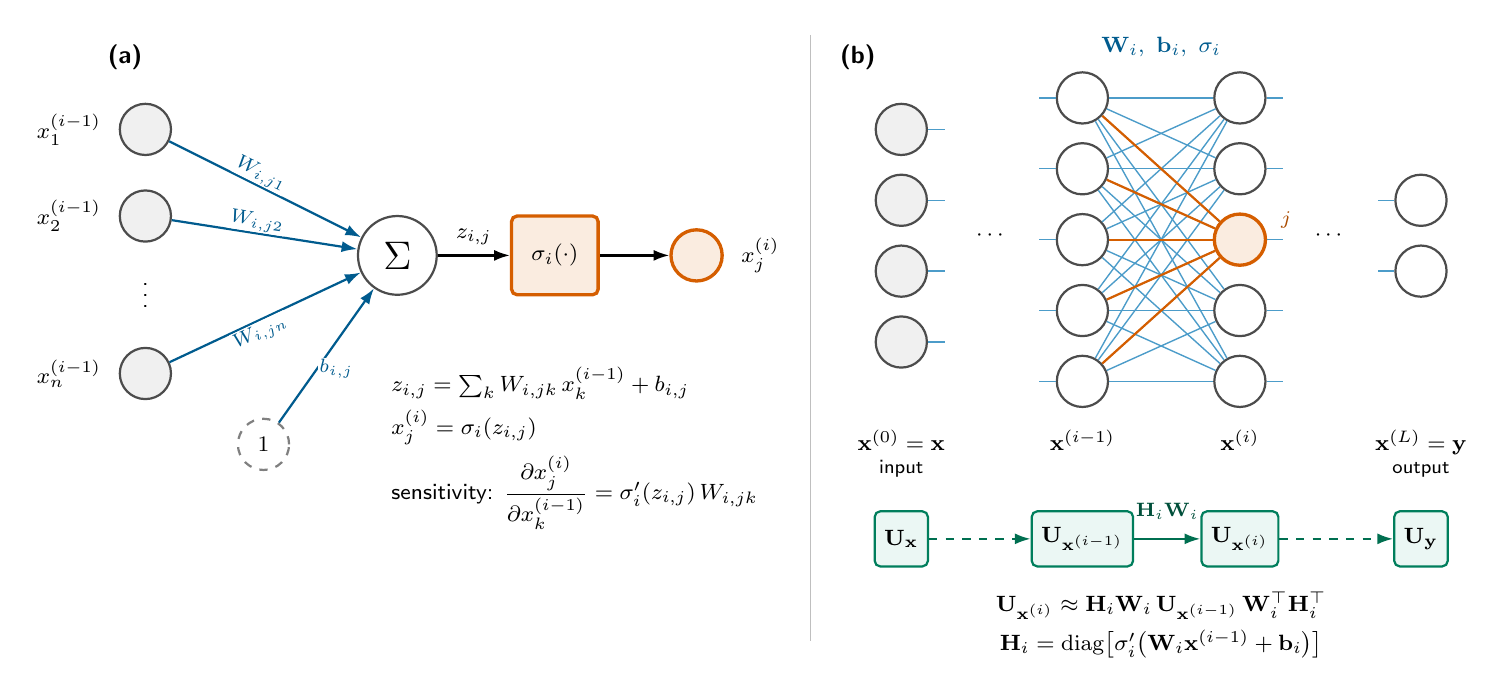
\begin{tikzpicture}[
  font=\sffamily\footnotesize,
  neuron/.style={circle, draw=black!70, thick, fill=white, minimum size=6.5mm, inner sep=0pt},
  input/.style={circle, draw=black!70, thick, fill=black!6, minimum size=6.5mm, inner sep=0pt},
  hl/.style={circle, draw=okOrange, very thick, fill=okOrange!12, minimum size=6.5mm, inner sep=0pt},
  edge/.style={draw=okBlue!70, line width=0.5pt},
  arrow/.style={-{Latex[length=2mm,width=1.4mm]}, thick},
  wlbl/.style={font=\scriptsize, text=okBlue!80!black, fill=white, inner sep=0.5pt},
  panel/.style={font=\sffamily\small\bfseries, anchor=north west},
  cov/.style={rectangle, rounded corners=2pt, draw=okGreen!80!black, thick, fill=okGreen!8,
    minimum height=7mm, inner sep=1.2mm},
  covarrow/.style={-{Latex[length=2mm,width=1.4mm]}, thick, draw=okGreen!70!black}
]

% =====================================================================
% (a) artificial neuron j of layer i
% =====================================================================
\begin{scope}
  \node[panel] at (-0.6,3.4) {(a)};
  % inputs x_k^(i-1)
  \foreach \k/\lab/\y in {1/1/2.2, 2/2/1.1, 3/n/-0.9} {
    \node[input] (in\k) at (0,\y) {};
    \node[left=1mm of in\k] {$x^{(i-1)}_{\lab}$};
  }
  \node at (0,0.2) {$\vdots$};
  % bias
  \node[input, fill=white, draw=black!50, dashed] (bias) at (1.5,-1.8) {$1$};
  % summation and activation
  \node[circle, draw=black!70, thick, fill=white, minimum size=10mm] (sum) at (3.2,0.6) {\Large$\Sigma$};
  \node[rectangle, rounded corners=2pt, draw=okOrange, very thick, fill=okOrange!12,
        minimum width=11mm, minimum height=10mm] (act) at (5.2,0.6) {$\sigma_i(\cdot)$};
  \node[hl] (out) at (7.0,0.6) {};
  \node[right=1mm of out] {$x^{(i)}_{j}$};

  \draw[arrow, okBlue!80!black] (in1) -- node[wlbl, pos=0.45, above, sloped] {$W_{i,j1}$} (sum);
  \draw[arrow, okBlue!80!black] (in2) -- node[wlbl, pos=0.45, above, sloped] {$W_{i,j2}$} (sum);
  \draw[arrow, okBlue!80!black] (in3) -- node[wlbl, pos=0.45, below, sloped] {$W_{i,jn}$} (sum);
  \draw[arrow, okBlue!80!black] (bias) -- node[wlbl, right, pos=0.4] {$b_{i,j}$} (sum);
  \draw[arrow] (sum) -- node[above] {$z_{i,j}$} (act);
  \draw[arrow] (act) -- (out);

  % equations under the neuron
  \node[align=left, anchor=north west, font=\sffamily\footnotesize] at (3.0,-0.7) {%
    $z_{i,j} = \sum_{k} W_{i,jk}\, x^{(i-1)}_k + b_{i,j}$\\[1mm]
    $x^{(i)}_j = \sigma_i\!\left(z_{i,j}\right)$\\[1mm]
    sensitivity: $\dfrac{\partial x^{(i)}_j}{\partial x^{(i-1)}_k} = \sigma_i'(z_{i,j})\, W_{i,jk}$};
\end{scope}

% =====================================================================
% (b) multilayer perceptron and layer-wise covariance propagation
% =====================================================================
\begin{scope}[xshift=9.6cm]
  \node[panel] at (-0.9,3.4) {(b)};
  % layer x-positions
  \def\xa{0}    % x^(0)
  \def\xb{2.3}  % x^(i-1)
  \def\xc{4.3}  % x^(i)
  \def\xd{6.6}  % x^(L)
  % input layer x^(0) = x
  \foreach \n/\y in {1/2.2,2/1.3,3/0.4,4/-0.5} \node[input] (A\n) at (\xa,\y) {};
  % layer i-1
  \foreach \n/\y in {1/2.6,2/1.7,3/0.8,4/-0.1,5/-1.0} \node[neuron] (B\n) at (\xb,\y) {};
  % layer i (neuron j highlighted)
  \foreach \n/\y in {1/2.6,2/1.7,4/-0.1,5/-1.0} \node[neuron] (C\n) at (\xc,\y) {};
  \node[hl] (C3) at (\xc,0.8) {};
  \node[font=\scriptsize, text=okOrange!80!black, right=0.5mm of C3, yshift=2.5mm] {$j$};
  % output layer x^(L) = y
  \foreach \n/\y in {1/1.3,2/0.4} \node[neuron] (D\n) at (\xd,\y) {};

  % full connections i-1 -> i
  \foreach \a in {1,...,5} \foreach \b in {1,...,5} \draw[edge] (B\a) -- (C\b);
  % emphasise the weights into neuron j
  \foreach \a in {1,...,5} \draw[draw=okOrange, line width=0.8pt] (B\a) -- (C3);
  % elided layers: short stubs and dots
  \foreach \a in {1,...,4} \draw[edge] (A\a) -- ++(0.55,0);
  \foreach \b in {1,...,5} \draw[edge] (B\b) -- ++(-0.55,0);
  \node at ($(\xa,0.85)!0.5!(\xb,0.85)$) {$\cdots$};
  \foreach \a in {1,...,5} \draw[edge] (C\a) -- ++(0.55,0);
  \foreach \b in {1,2} \draw[edge] (D\b) -- ++(-0.55,0);
  \node at ($(\xc,0.85)!0.5!(\xd,0.85)$) {$\cdots$};

  % parameters of layer i
  \node[font=\footnotesize, text=okBlue!80!black] at ($(\xb,3.25)!0.5!(\xc,3.25)$)
    {$\mW_i,\ \vb_i,\ \sigma_i$};

  % layer labels
  \node[anchor=north, align=center] at (\xa,-1.5) {$\vx^{(0)} = \vx$\\[-0.5mm]{\scriptsize input}};
  \node[anchor=north, align=center] at (\xb,-1.5) {$\vx^{(i-1)}$};
  \node[anchor=north, align=center] at (\xc,-1.5) {$\vx^{(i)}$};
  \node[anchor=north, align=center] at (\xd,-1.5) {$\vx^{(L)} = \mathbf{y}$\\[-0.5mm]{\scriptsize output}};

  % covariance propagation row
  \node[cov] (U0) at (\xa,-3.0) {$\mU_{\vx}$};
  \node[cov] (U1) at (\xb,-3.0) {$\mU_{\vx^{(i-1)}}$};
  \node[cov] (U2) at (\xc,-3.0) {$\mU_{\vx^{(i)}}$};
  \node[cov] (U3) at (\xd,-3.0) {$\mU_{\mathbf{y}}$};
  \draw[covarrow, dashed] (U0) -- (U1);
  \draw[covarrow] (U1) -- node[above=1.2mm, font=\scriptsize, text=okGreen!50!black] {$\mH_i\mW_i$} (U2);
  \draw[covarrow, dashed] (U2) -- (U3);
  \node[anchor=north, font=\footnotesize, align=center] at ($(\xa,-3.0)!0.5!(\xd,-3.0)+(0,-5.5mm)$)
    {$\mU_{\vx^{(i)}} \approx \mH_i\mW_i\,\mU_{\vx^{(i-1)}}\,\mW_i^{\top}\mH_i^{\top}$\\[1mm]
     $\mH_i = \operatorname{diag}\!\left[\sigma_i'\!\left(\mW_i\vx^{(i-1)} + \vb_i\right)\right]$};
\end{scope}

% panel separator
\draw[black!25] (8.45,3.4) -- (8.45,-4.3);

\end{tikzpicture}%
\end{lrbox}%
% crop the page to the picture
\pdfpagewidth=\dimexpr\wd\figbox+2\figborder\relax
\pdfpageheight=\dimexpr\ht\figbox+\dp\figbox+2\figborder\relax
\pdfhorigin=\figborder
\pdfvorigin=\figborder
\shipout\hbox{\usebox{\figbox}}
\end{document}
